\documentclass{easychair}

\usepackage{amssymb,amsmath,mathtools,empheq,fancybox}

\usepackage{paralist}
\usepackage{url}
\usepackage{color}

\usepackage{textcomp,listings}
\usepackage{biblatex}
\usepackage{mymacros}
\usepackage{mathpartir}
\usepackage{csquotes}
\usepackage[font={small,it}]{caption}
\addbibresource{../bibliography.bib}



\newif\ifcomments
\commentstrue

\newcommand{\pr}[1]{{\color{red}``PR: #1''}}
\newcommand{\as}[1]{{\color{blue}``AS: #1''}}

\newif\ifoutline
\outlinetrue

\newcommand{\contents}[1]{\ifoutline{\color{blue}
    \begin{itemize}
    #1
    \end{itemize}
  }\fi}

\allowdisplaybreaks[1]
\title{A Solver for Generalised Parikh Images of Regular Languages}
\author{Amanda Stjerna \and Philipp Rümmer}
\institute{Uppsala University, Sweden}

\begin{document}
\maketitle

\section{Introduction}

Parikh images have a wide application within automata, including for the solving
of string constraints in automata-based solvers such as \Ostrich{}
\cite{ostrich}. While it is possible to compute the Parikh image of an automaton
by adapting the method for CFGs of~\cite{generate-parikh-image}, this method
produces clauses with many existentially quantified variables which are costly
to eliminate. This makes many real-world applications intractable. Furthermore,
applications like Unicode require automata with symbolic labels to handle their
large alphabets, increasing the number of variables even more.
Finally, automata-based string solvers compute Parikh images on products of
automata, derived from conjunctions of string constraints. Using
\cite{generate-parikh-image} this would require the up-front computation of the
product before its Parikh image, running the risk of an exponential blow-up.

Addressing these concerns, we introduce a lazy approach to the computation of
Parikh images of products of automata that also generalises operations on
labels. This allows us to extend the computation of Parikh images to handle
symbolic transition labels ergonomically, while also allowing us to interleave
the computations of the Parikh image of a product and the product itself. This
allows both calculations to inform each other, thereby eliminating unnecessary
work. Moreover, the scheme allows us to learn interesting facts (in the form of
implied clauses) about the problem.

Based on these insights, we present a work-in-progress tool to solve linear
constraints on symbolic automata with counters, aka Parikh automata, amounting
to constraints on the Parikh image of their product. We are able to generate
both a Presburger formula representing the image and find satisfying assignments
within it.

\section{Background}

Formally, the \textit{Parikh map} over a context-free language $\Sigma = \left\{a_1, \ldots, a_k \right\}$ is defined as in \cite{kozen}:

$$
\begin{aligned}
& \psi: \Sigma^* \rightarrow \mathbb{N}^k \\
& \psi(s) = \left[\#a_1(s), \#a_2(s), \ldots, \#a_k(s)\right]
\end{aligned}
$$

That is, $\psi(s)$ is a vector of the number of occurrences of each character in the language for a given string $s$. For example, for  $\Sigma = \left \{ a, b\right\}$, we would have $\psi(abb) = \left[1, 2\right]$.

We define the image of this map, the \textit{Parikh image}, of some subset of the language $A \subseteq \Sigma^*$ as:

$$
\psi(A) = \left\{ \psi(x) | x \in A \right\}
$$

Thus, we would have $\psi(\left\{ab, abb\right\}) = \left\{\left[1, 1\right], \left[1, 2\right]\right\}$. An interesting property of this map is that it can always be expressed as a symbolic Presburger formula.

\subsection{Generalised Parikh Images}\label{sec:generalised}

Another way of viewing the Parikh map is as a monoid homomorphism $p:\: \left(\Sigma^*, \cdot, \epsilon \right) \to (\mathbb{Z}^\Sigma, +, \vec{0})$, where $\cdot$ is the string concatenation operation, the objects of the right-hand-side monoid are character counts, and $+$ is element-wise vector addition. Note that while the left monoid does not commute, the right one does.

This viewpoint enables us to generalise the Parikh map further to arbitrary monoid morphisms $h:\: \Sigma^* \to M$ where $M$ is a commutative monoid. It then follows from the universal mapping property that any such morphism $h$ can also be expressed in terms of the Parikh map, as $h' \circ p$.

An example is computing the length of a string, which is expressed in terms of
the Parikh map by summing the individual character counts of the vector: $h':\:
(\mathbb{Z}^\Sigma, +, \vec{0}) \to (\mathbb{Z}, +, 0) = \vec{x} \to \sum_{i \in
\Sigma} x_i$. More generally, this approach extends to multiple counters to
produce Parikh automata with one such counter per symbol in the language, as
used in implementations of many string
constraints~\cite{path-feasibility-strings}.

\section{Lazy Computation of Parikh Images for Regular Languages}
The calculus is based on four principles: linear equations to preserve flow
through the automaton, case-splitting when there are multiple possible paths a
run can take, propagation of connectedness constraints, and materialisation of
products. Notably, ensuring connectedness of a run in the presence of cycles is
the computationally most difficult constraint to enforce, as the flow equations
of any loop will self-balance.

Starting with the automaton shown to the left in figure~\ref{fig:automaton}, we
seek a satisfying assignment as an illustration of our calculus.


\begin{figure}[h]
  \caption{Left to right: the starting automaton, the automaton with its corresponding linear equations, and the solution. Note the replacement of the existentially quantified transition variables with character count constants, and the introduction of a linear equation across the edge for \texttt{d} representing a choice between either an~\texttt{a} or a~\texttt{d}. Transitions with a zero value are not used in the solution.}\label{fig:automaton}
  \begin{minipage}[t]{0.3\textwidth}
    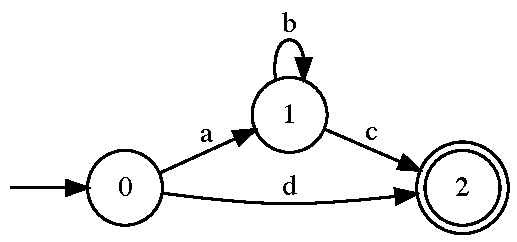
\includegraphics[width=\textwidth]{trace-0}
    \end{minipage}
    \begin{minipage}[t]{0.3\textwidth}
    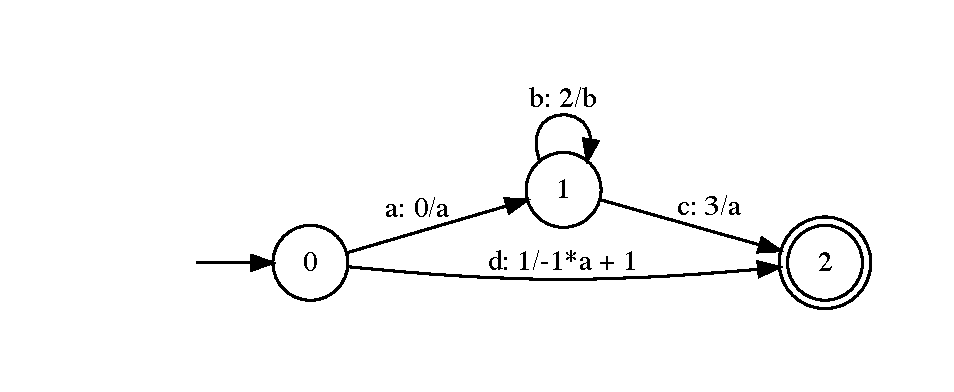
\includegraphics[width=\textwidth]{trace-0-aut-0}
    \end{minipage}
    \begin{minipage}[t]{0.3\textwidth}
      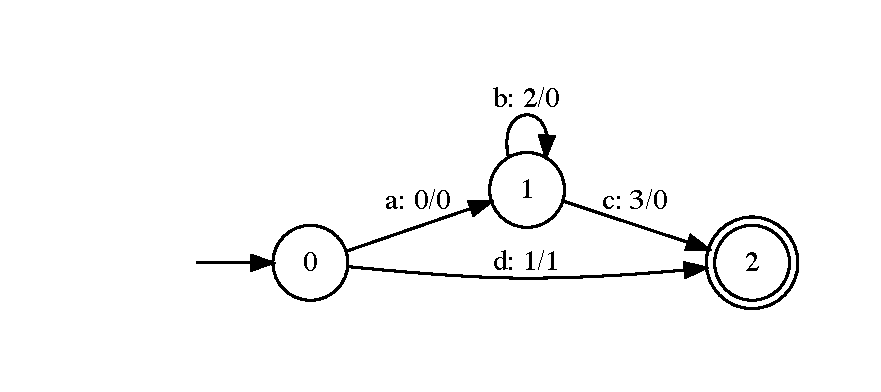
\includegraphics[width=\textwidth]{trace-3-aut-0}
      \end{minipage}
  \end{figure}

  In this case, our calculus will introduce a free integer constant per
  character ($a$, $b$, $c$, and $d$). It will then introduce equations
  preserving flow through the automaton corresponding to how many times that
  transition is used in a run. Each transition will be given an
  existentially quantified variable in these equations, and each of our target
  variables is constrained to the sum of the transitions where it occurs as a
  label. This corresponds to the first portion of the formula described
  in~\cite{generate-parikh-image}, but crucially misses the constraints to
  ensure connectedness in the presence of cycles. Instead, we enforce this
  constraint lazily.

  Note that this formulation allows us to propagate information between terms of
  a product before materialising it to exclude infeasible parts of a product from the computation.
  
Before computation begins, our prover performs reasoning on the flow equations
to simplify them into $d + a = 1 \land c = a$. This leaves us with a choice of
two paths for our run so we execute a case split: \textsc{Split}: $a \leq 0$
$\mid$ $a > 0$. The split is performed as close to the initial state as possible
and favours deselecting an edge by constraining its corresponding term to be 0.
The linear inequalities of the flow equations will ensure that the choice
selects precisely one of the upper and lower paths.

Since choosing the \texttt{d}~transition over \texttt{a} disconnects a loop, the \texttt{b}~transition, from the initial state, we evaluate the rule \textsc{Propagate-Connected} to add the constraint $b = 0$ and exclude the unreachable \texttt{b} from our run. Afterwards we can subsume the propagator for the connectedness constraint as all loop transitions terms are negative, and our run is therefore guaranteed to be connected. This leaves us with an automaton with just one nonzero transition, as seen in the rightmost image of figure~\ref{fig:automaton}.

As there is just one automaton left, there are no products to materialise and so
the calculation is complete. We present the assignment $a = b = c = 0, d=1$. To
find the Parikh image rather than an assignment, we would iteratively query
our calculus for partial solutions and perform quantifier elimination on the
free constants.

%\bibliographystyle{splncs03}
\printbibliography

\end{document}
